\documentclass{beamer}
\usepackage{cancel, algpseudocode, hyperref, tikz, venndiagram, centernot}

\title{CS 70 Discussion 12B}
\date{November 22, 2024}

\begin{document}

\frame{\titlepage}

\begin{frame}
    \frametitle{Normal/Gaussian Distribution}
    {\bf Problem}: What are we referring-to when we are talking about the ``bell curve''?\\
    {\bf Solution}: We have a continuous distribution known as the {\bf Gaussian distribution} or {\bf normal distribution}. The PDF of a normal distribution of mean $\mu$ and {\bf standard deviation} $\sigma$ looks like the following:
    \begin{center}
        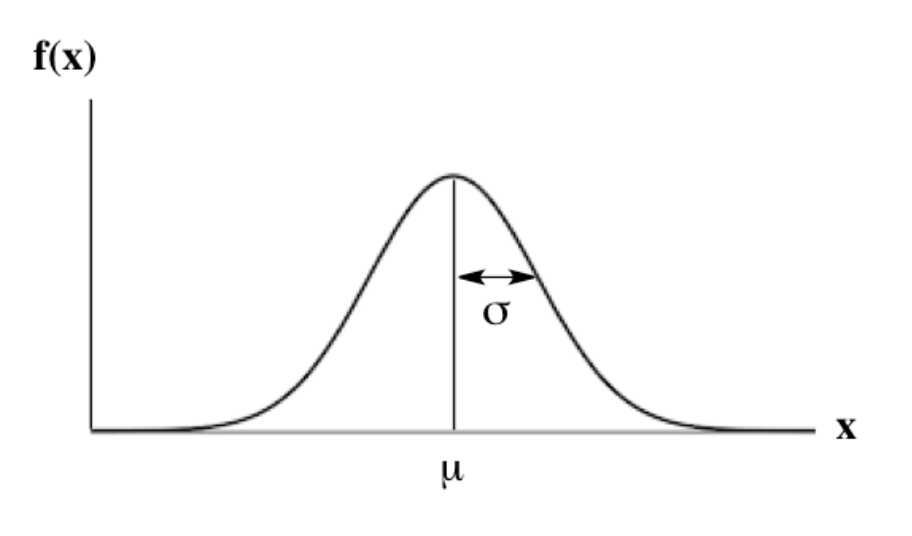
\includegraphics[scale=0.5]{Images/normal-distribution.png}
    \end{center}
\end{frame}

\begin{frame}
    \frametitle{Normal/Gaussian Distribution (Cont.)}
    For some Gaussian random variable $X$, the following always hold:
    \begin{itemize}
        \item Notation: $X$ being Gaussian with expectation $\mu$ and standard deviation $\sigma$ is denoted as $X\sim\mathcal{N}(\mu,\sigma^2)$.
        \item Standard Normal Distribution: $X$ following a {\bf standard normal distribution} is denoted as $X\sim\mathcal{N}(0,1)$.
        \item PDF of $X$:
        \begin{align*}
            f_X(x)=\frac{1}{\sigma\sqrt{2\pi}}\text{exp}\left(-\frac{1}{2\sigma^2}(x-\mu)^2\right)
        \end{align*}
        \item CDF: There is actually no closed-form CDF formula for a Gaussian distribution, and we only have approximations. We commonly denote the CDF for a standard Gaussian as $\Phi(x)$, and:
        \begin{align*}
            F_X(x)=\Phi\left(\frac{x-\mu}{\sigma}\right)
        \end{align*}
    \end{itemize}
\end{frame}

\begin{frame}
    \frametitle{Normal/Gaussian Distribution (Cont.)}
    For Gaussian random variable $X$, the following also always hold:
    \begin{itemize}
        \item $X\sim\mathcal{N}(\mu,\sigma^2)$ implies $\frac{X-\mu}{\sigma}\sim\mathcal{N}(0,1)$
        \item For constants $a$ and $b$, $X\sim\mathcal{N}(\mu,\sigma^2)$ implies:
        \begin{align*}
            aX+b\sim\mathcal{N}(a\mu+b,a^2\sigma^2)
        \end{align*}
        \item For constants $a$ and $b$, two independent Gaussians $X\sim\mathcal{N}(\mu_1,\sigma_1^2)$ and $Y\sim\mathcal{N}(\mu_2,\sigma_2^2)$ follow:
        \begin{align*}
            aX+bY\sim\mathcal{N}(a\mu_1+b\mu_2,a^2\sigma_1^2+b^2\sigma_2^2)
        \end{align*}
    \end{itemize}
\end{frame}

\begin{frame}
    \frametitle{Central Limit Theorem (CLT)}
    {\bf Problem}: When I have a distribution that is defined as the sum of $n$ {\bf independent, identically-distributed (i.i.d.)} trials, why does it look like a Normal distribution?\\
    {\bf Solution}: Let's consider some random variable $S_n=\sum_{i=1}^nX_i$, where each $X_i$ are i.i.d. with mean $\mu$ and variance $\sigma^2$. The {\bf Central Limit Theorem (CLT)} says that as $n\rightarrow\infty$:
    \begin{align*}
        \frac{S_n-n\mu}{\sigma\sqrt{n}}\rightarrow\mathcal{N}(0,1)\text{ and }\frac{\frac{1}{n}S_n-\mu}{\frac{\sigma}{\sqrt{n}}}\rightarrow\mathcal{N}(0,1)
    \end{align*}
    This means that the {\bf standardized} form of the distribution $S_n$ (i.e. $\frac{S_n-\mathbb{E}[S_n]}{\sqrt{\text{Var}(S_n)}}$) looks more and more like the standard normal distribution as $n$ grows larger. Therefore, for large $n$, we can use $\Phi$ to approximate probabilities of $S_n$ taking certain values.
\end{frame}

\end{document}
